\chapter{Data Extraction} \label{chapter:data-extraction}
In order to draw any conclusions regarding the relationship of bond and stock returns, the respective static and time series data needs to be acquired first. Since equity data is already available from the beginning of the IDP, the bond data is the only one which had to be acquired. For bond data extraction, the financial database product Datastream, provided by Thomson Reuters, can be used, since it is licensed for usage by TUM students and employees. 

\section{Download Solution} \label{section:download-solution}
As Thomson Reuters has a wide range of products which can be used for different types of data, the first thing that needed to be done, was to determine the most suitable product to download both static and time series data for corporate bonds. After some time spent reading up and gathering information on the Thomson Reuters product portfolio, it became apparent that some of the products, such as the TR Python API, are only suitable for equity data download, and not for corporate bonds, and only have a very limited number of parameters available for download. On the other hand, it was found that other Thomson Reuters products, which would normally be suitable for automated download of bond data, such as e.g. DataScope Select (DSS) or Thomson Reuters Tick History (TRTH), are not included in the existing academic license. Other products -- noticeably the Datastream Web Service (DSWS) API, which is most suited for such requests -- are generally not available for academic clients. 

These findings were a significant setback for the bond data extraction, since the only option left to acquire large amounts of corporate bond data, was over the Datastream Add-In for Microsoft Excel. While this add-in is rather convenient for small-scale manual requests with the help of so-called request tables, it is not optimized for large data extraction queries. It does not provide an API for customizable requests. Instead, communication with the Datastream server is handled over a single API call available in VBA. This one and only callable function is implemented in C++, and can only be invoked in a black-box manner, since the provider does not give out its implementation. This leads to only one possible solution to automatically extract corporate bond data from Datastream. It can be described with the following steps: 
\begin{enumerate}
		\item Acquire Datastream codes / identifiers for all financial instruments which need to be downloaded.
		\item Split these identifiers into batches small enough to be processed in a single Datastream request.
		\item Fill a request table with as many requests as needed to include all the batches. 
		\item Launch the Datastream requests for all the batches one after the other. 
		\item Monitor the download process to ensure that the data is being consistently downloaded. 
\end{enumerate}
The programmatic development of the download tool will be based exactly on these five steps. The last step (monitoring the execution) is especially crucial and complex to implement. The reason for this is, as previously mentioned, that the Datastream Excel Add-In is not well-fit for large data downloads. Therefore, the following problems continuously arise during the download process: 
\begin{itemize}
	\item Datastream add-in eventually signs out for no obvious reason. 
	\item Data download hangs, without any notification stating the reason or the hanging fact itself. 
	\item Excel suspends the add-in and places it into a blacklist for repeated faulty behavior. 
\end{itemize}
Since VBA is single threaded and cannot detect or react to erroneous behavior when the download is running, it is impossible to do the monitoring in the VBA/Excel environment. For this purpose, a Python wrapper was developed as will be explained in \ref{section:error-monitor}.

\section{Bond Identifiers Acquisition} \label{section:bond-identifiers-acquisition}
Since for both static and time series requests Datastream requires unique financial instrument codes to be provided, it is first necessary to obtain a list of identifiers for the securities for which the data needs to be downloaded. The most commonly used unique security identifier in Datastream is the so-called Datastream Code (short \textit{dscd}). In the scope of the project two different approaches have been developed for this task, and will be introduced in the following. 

\subsection{Programmatic Identifier Extraction}
For the purpose of this work, we are interested in corporate bonds from all possible jurisdictions, and with any possible coupon an currency parameters. The only restriction is that we only concentrate on the issue date range between Dec 31, 1999 and June 30, 2020 (date of extraction). 

Datastream allows to filter its financial security dataset by these parameters, e.g. when clicking on \textit{Find Series} in a request table. After the securities have been filtered for the desired corporate bonds, these can be selected by repeatedly checking the box to select all bonds on the current page, and then clicking on \textit{Next} to switch to next page. This is due to Datastream not providing an option to select all filtered securities at once if there are more than 4,000. Hence, if there are for instance 60,000 corporate bonds in the database in total, one would not be able to select them all at once. Instead, one would have to select the 15 bonds on the current page and then switch to next page $60,000 / 15 = 4,000$ times. This is of course very cumbersome for the user, and the repeated clicking sounds like a good process to automate programmatically. 

There are multiple tools and scripting languages which enable fast and easy click automation. Specifically for this project I decided to go with Python 3 for this purpose, since it was already part of the environment. One of the packages which enable GUI automation in Python is \textit{pyautogui}\footnote{https://pyautogui.readthedocs.io/en/latest/}. 
With build-in methods like $click()$ and $hotkey()$ it enables the user to simulate mouse clicks on the computer screen by giving the functions the screen coordinates of the buttons. Placing the commands into a loop in the right order makes it possible to simulate the entire process of selecting corporate bonds in Datastream. For a possible Python implementation see the file \textit{datastream\_pyautogui.py} in the project files. Note that the screen coordinates can significantly differ depending on the screen resolution and window settings. 

While the described approach solves the problem of selecting all the needed corporate bonds from Datastream, there are two downsides to it. The first one is that it is cumbersome for the developer to determine and to enter the screen coordinates of all the buttons involved. The second is that, even when fully automated, the tool needs a lot of time to select and return all of the chosen securities if there are many of them. At this point, the second approach, even though it is manual, is both faster and easier to apply. 

\subsection{Manual Identifier Extraction}
To extract the needed corporate bond identifiers manually, we can make use of the fact that Datastream allows to select all filtered securities at once when there are less than 4,000. Because of this, we can simply split our entire data into multiple chunks that are all smaller than 4,000 bonds in total. This can be done by selecting one or more parameters (the number depends on the size of the dataset) according to which the bonds can be filtered even further. For example, an entire bond dataset with 60,000 bonds in total can be split by coupon size first, and then additionally by currency to produce bond batches of maximum 4,000 bonds each. For a visualization of this approach, see Fig. \ref{fig:bond-splitting}. 
\begin{figure}[h]
	\centering
	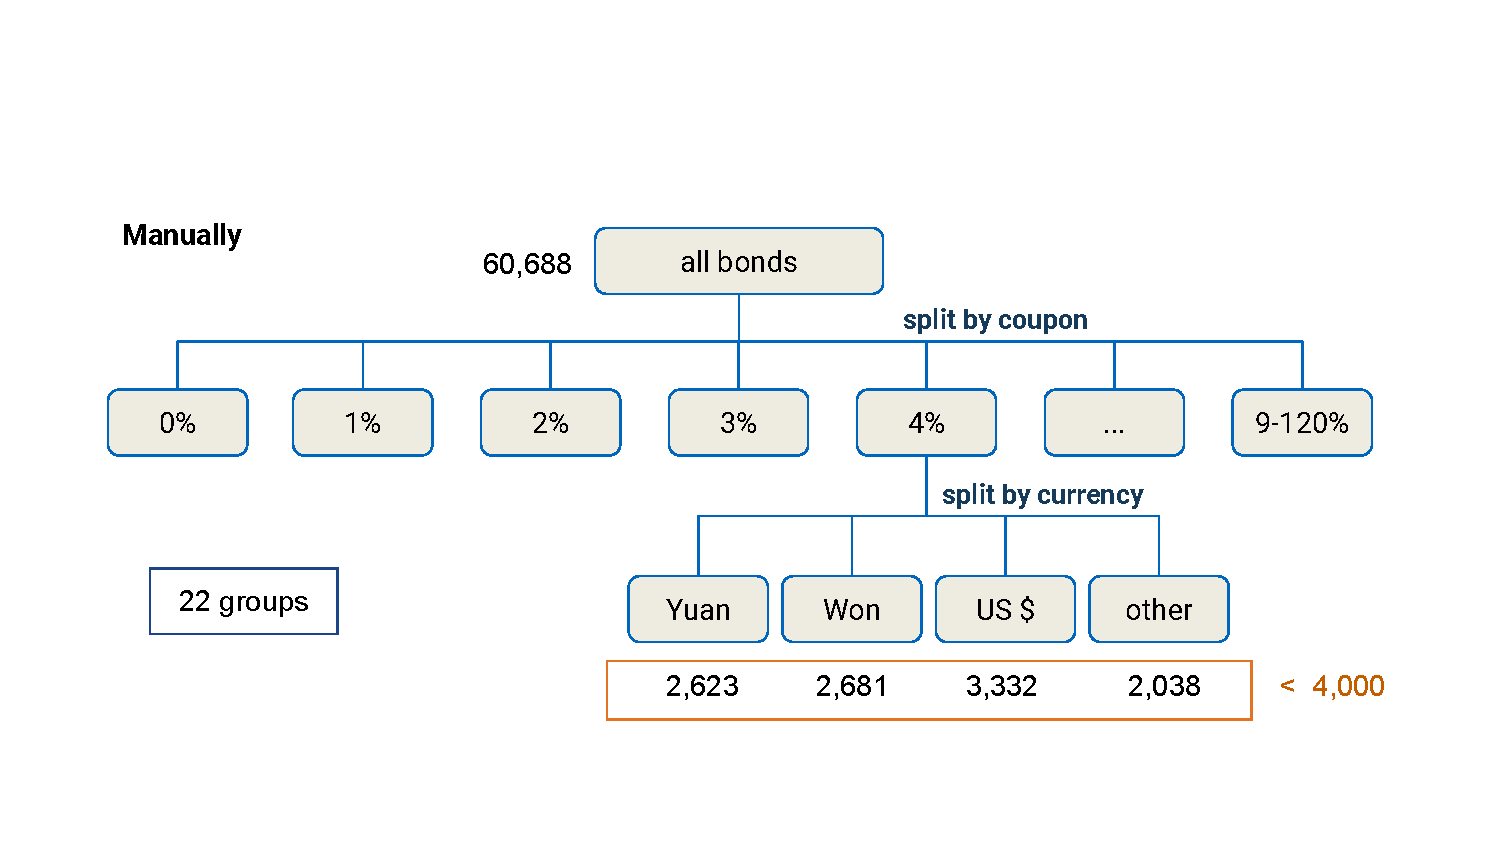
\includegraphics[trim={0 2cm 0 3cm},clip,width=1.0\linewidth]{figures/bond-splitting}
	\caption{Bond split by coupon and currency}
	\label{fig:bond-splitting}
\end{figure}
If the split has been done properly, it will include all of the desired securities, since each bond belongs to one particular coupon size as well as currency group. In most cases, there will be only few groups that need to be extracted from the interface. In the case of 60,000 bonds, one would only have $60,000 / 4,000 = 15$ groups in total. In reality, for this concrete use case, 19 different bond groups had to be created. This is because not all splits are perfect, and some of them just consist of 3,500 bonds instead of 4,000 for example. After the splitting work has been done, the resulting bond groups can be extracted manually with just a few clicks. 

\section{Automating the Request Table} \label{section:automating-request-table}
After the bond identifiers in form of \textit{dscd} codes have been extracted, they can be used to retrieve both static and time series data from Datastream. For this purpose, I wrote a VBA program which fully automates the download process. The only input needed from the user is the \textit{dscd }identifiers, the desired variable codes (such as price, issued volume, etc.) as well as the desired time frames in the case of a time series request. Since the program code is rather complex, I will only cover the main approach briefly. A more in-depth description can be found in appendix \ref{appendix:technical-aspects} to this work. 

At the beginning, the VBA tool retrieves the user-provided identifiers and datatypes from the respective Excel files. Then, based on the input size, multiple calculations take place. For static information requests not much needs to be done, since these are usually relatively small and only depend on the number of securities for which the data is requested. For time series requests though, the tool estimates how large the entire request will get, depending on dates window, frequency of time points (e.g. daily or quarterly), the number of datatypes, and the number of identifiers. If the request is too large to be processed by Datastream in one run, it gets split into multiple smaller requests of equal size. Since there is no particular metric to estimate in advance whether a particular request will be executed by Datastream, or whether it is too large for that, the tool only computes an approximation based on an empirically measured \textit{Bytes per Field} metric. The single requests then get entered into the request table one below the other, and each receive an own Excel file as destination to store the data. 

As soon as the request table has been filled (which does not take long), the command to process the first request is issued to Datastream. This happens via a call to the single available function, which tells Datastream to process the current request table in a black-box manner. After the request ends, the tool checks whether the requested data has arrived to the destination file. If not, it checks the connection of the Datastream add-in and issues a warning to the user if the add-in unexpectedly disconnected. In both cases, the result of the request is logged, in order for the user to be able to read up on the proceedings later. To prevent the computer from sleeping or going in idle mode, the tool moves the computer mouse pointer after each request with a dedicated VBA function. When the first request of the request table has been processed, the other ones get executed in the same manner one after the other. Note that while it is possible to submit the execution for all requests at once, it is not advisable, since Datastream might issue an error due to the data being too large, or might otherwise simply hang during execution. This is exactly the reason why we had to split up the original request in multiple parts in the first place. 

While the entire Datastream Extraction Tool is much more complex than what has been described here, the given explanation covers the most crucial parts of the download process. At this point, note that the error monitoring step, which was previously mentioned as essential, cannot be completed in VBA due to its single-threaded execution engine. Section \ref{section:error-monitor} will cover the required workaround for this functionality. 

\section{User Interface} \label{section:user-interface}
In order to provide a graphical user interface as well as an error monitoring capacity (section \ref{section:error-monitor}) for the created VBA tool, a Python 3 wrapper program has been created. It's architecture can be seen in Fig. \ref{fig:ds-extraction-tool-architecture}. At this point, note that a detailed usage manual for the Datastream Extraction Tool -- including its user interface -- can be found in appendix \ref{appendix-dset-manual} to this work.

\begin{figure}[h]
	\centering
	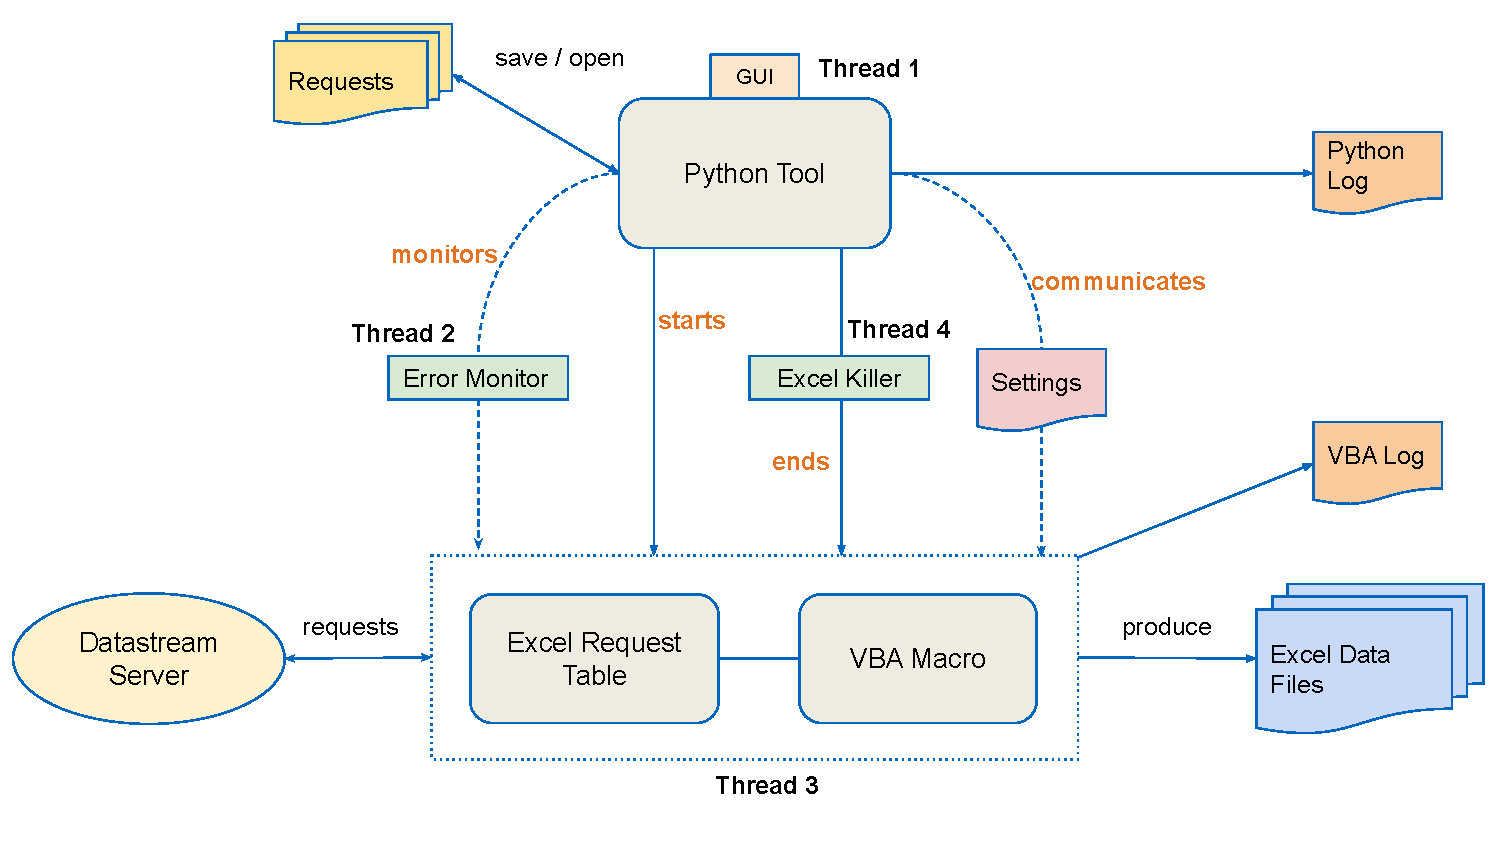
\includegraphics[width=1.1\linewidth]{figures/ds-extraction-tool-architecture}
	\caption{Architecture of the Datastream Extraction Tool}
	\label{fig:ds-extraction-tool-architecture}
\end{figure}

As shown in the visualization, the Python program has a \textit{GUI} component, which runs on its main thread (Thread 1). The layout of the user interface is depicted in Fig. \ref{fig:gui}. 

\begin{figure}[h]
	\centering
	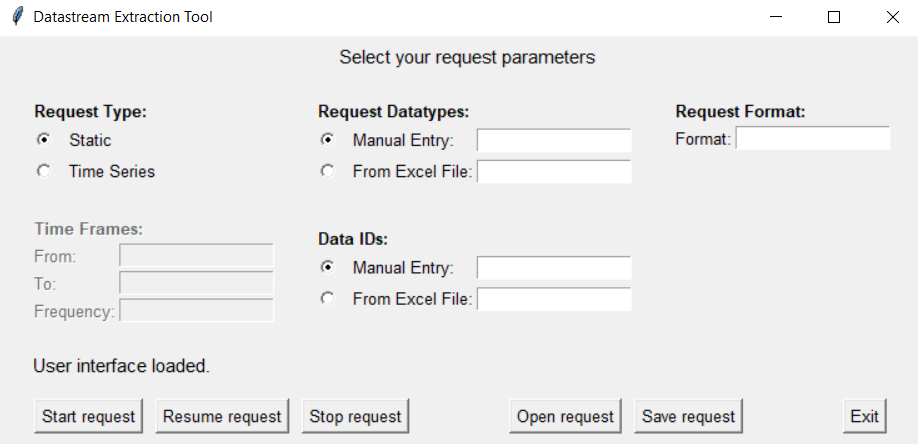
\includegraphics[width=1.1\linewidth]{figures/gui.png}
	\caption{Graphical User Interface of the Datastream Extraction Tool}
	\label{fig:gui}
\end{figure}

Its features include: 
\begin{itemize}
	\item Request type selection (static or time series)
	\item Time frames and frequency for time series requests
	\item Request datatypes, which can be entered either in a manual list or via an Excel file
	\item Data identifiers, which can also be entered either manually or via Excel file
	\item Request format with one or more Datastream request options (e.g. header row, currency, etc.)
	\item Destination choice for downloaded data
	\item Saving and reusing frequently entered requests
\end{itemize}

The user interface has been programmed using the \textit{Tkinter}\footnote{\url{https://docs.python.org/3/library/tkinter.html}} package, which enables rudimentary container-based gui creation. 

\section{Other Functionality} \label{section:other-functionality}
Besides the user interface, the Python wrapper offers a logging facility for the actions taken, as well as a functionality to exchange settings and messages with the VBA component. For the latter purpose, a \textit{settings.txt} file is provided which encompasses user-provided request details to forward the request to the VBA program. The entries are made in a key-value manner, which enables a fast and easy information exchange between the Python and the VBA parts. Besides request forwarding, the settings file is used by the Python tool to receive regular updates from the VBA on the current download status. This information is used for both status updates within the gui as well as for the error monitoring functionality which will be explained in section \ref{section:error-monitor}. 

\section{Error Monitor} \label{section:error-monitor}
As shown in the visualization, the \textit{Error Monitor} module runs in a separate thread (Thread 2), since Python allows execution on multiple threads simultaneously. It is started from the main thread, which controls the graphical user interface, whenever a new download request (Thread 3) has been issued to Datastream. The module maintains an internal counter which signifies the waiting time for the current request in Datastream to process. The counter gets increased each time the Python tool notices that the currently processed request in VBA has not yet changed to the next one. VBA, in its turn, keeps posting updates on the number of the request that is currently being downloaded to the settings file. The ping frequency of the error monitor can be adjusted to the user needs, and is currently set to 1 minute cycle time. 

Whenever the counter of the error monitor reaches a programmer-defined threshold (currently 25 minutes), another component of the Python wrapper, the \textit{Excel Killer} (Thread 4) comes into play. It issues an operating-system-level command to (violently) terminate the currently running Excel process. The reason why this has to be done violently is that Excel becomes entirely non-responsive whenever the Datastream download is hanging. Therefore, asking Excel to exit nicely does not result in Excel shutting down. The terminate request needs to run on a separate thread so as to not interfere with the Python gui and status updater. 

After the current Excel process and thus also the running Datastream download have been shut down, the Python tool restarts the download request from the same point where it finished its download before it started hanging. In other words, the download request gets automatically resumed. 

Another functionality which the error monitor provides is the ability to detect when all needed data has been downloaded. This happens in a manner similar to the error monitoring itself. The tool simply reads in the number of the last executed download request from the settings file. Based on this information and on the total number of requests to be executed, it determines when the last data batch has been downloaded and ends the download. A corresponding status message is delivered to the user interface to notify the user that the download has finished. 

The entire Datastream Extraction Tool consisting of the VBA and Python parts, and including the required folder structure, is currently hosted on Google Drive under \url{https://bit.ly/3rB3lqg} -> \textit{Datastream Extraction Tool}.  


